\documentclass[12pt,a4paper]{report}

\usepackage[a4paper,top=3cm,bottom=3cm,left=3cm,right=3cm,marginparwidth=1.75cm]{geometry}

\usepackage[utf8]{inputenc}
\usepackage{amsmath}
\usepackage{amsthm}
\usepackage{amsfonts}
\usepackage{amssymb}
\usepackage{graphicx}
\usepackage[center]{caption}
\usepackage{bussproofs}
\usepackage[italian]{babel}
\usepackage{fancyhdr}
\usepackage{verbatim}
\usepackage{afterpage}
\usepackage[shortlabels]{enumitem}

\usepackage{graphicx}
\graphicspath{ {./images/} }

\pagestyle{fancy}
\fancyhf{}
\fancyhead[LE,RO]{\thepage}
\fancyhead[RE]{ \nouppercase \leftmark}
\fancyhead[LO]{ \nouppercase \rightmark}

\theoremstyle{plain}
\newtheorem{thm}{Teorema}[chapter] % reset theorem numbering for each chapter
\theoremstyle{definition}
\newtheorem{lemma}{Lemma}[chapter]
\newtheorem{defn}{Definizione}[chapter]
\newtheorem{propr}{Proprietà}[chapter] 
\newtheorem{exmp}{Esempio}[chapter]

\linespread{1.2}
\parindent 10pt

\title{Relazione ElIVA}
\author{Daniele Pautasso}
\begin{document}
\begin{Large}
\begin{center}
\textbf{Relazione progetto ElIVA\\ \vskip 0.3cm Daniele Pautasso\\}
\end{center}
\end{Large}

\section*{Seam carving}
Il progetto realizzato è l'implementazione di una particolare operazione, detta seam carving. Le tradizionali tecniche per effettuare un retargeting dell'immagine sono solitamente cropping e scaling. Tuttavia, entrambe le strategie appena citate spesso non si rivelano ottimali: la prima consiste in una semplice operazione di ritaglio e pertanto in molti casi non è in grado di sintetizzare adeguatamente tutta l'informazione contenuta nell'immagine originale, mentre la seconda ne altera l'aspect ratio producendo immagini distorte e poco gradevoli per l'utente. Un approccio alternativo è stato proposto in [1]. L'idea di base è ridurre (aumentare) gradualmente le dimensioni di un immagine eliminando (introducendo) ad ogni iterazione un seam, ovvero un ``cammino" di pixel tra loro connessi e tale che esattamente un pixel sia scelto per ciascuna riga. Ovviamente per applicare suddetta operazione alle colonne è sufficiente ruotare l'immagine originale. La costruzione del seam è effettuata in base ad una misura che si propone di identificare gli elementi più rilevanti dell'immagine; così facendo quest'ultima viene alterata in modo tale da eliminare solo quelle parti che presentano un minore contenuto informativo, limitando allo stesso tempo le deformazioni tipiche dello scaling. 

\section*{Seam removal e seam insertion}
Prima di passare all'algoritmo vero e proprio occorre definire una qualche misura (nell'articolo viene detta ``energia") che possa assegnare a ciascun pixel una certa importanza.  Inizialmente come misura di energia è stata proposta la somma valori assoluti del gradiente. Se con I indichiamo l'immagine originale si ha 
\[ e(I) = | \frac{\delta I}{\delta x} | + | \frac{\delta I}{\delta y} |\]
Si attribuisce cioè importanza alle alte frequenze e di conseguenza agli edge, in quanto elementi costitutivi dell'immagine stessa. L'obiettivo del processo di seam removal è quindi trovare e rimuovere il percorso di pixel tra loro connessi la cui quantità di energia totale è minima.

In un articolo successivo ([2]) gli autori hanno perfezionato questa idea introducendo il concetto di forward energy: invece di rimuovere il percorso contenente la minor quantità di energia, la scelta ricade sul seam che, se rimosso, introduce meno energia. Questo permette di ottenere immagini in cui la presenza di artefatti dovuti alla rimozione o all'inserimento dei seam è meno accentuata.

Supponendo di procedere incrementando l'indice $i$, alla riga $i$-esima il pixel da aggiungere al seam potrà essere solo uno dei tre immediatamente sotto al pixel scelto al passo precedente. Il costo della rimozione del pixel di indice ($i,j$) è quindi dato da una funzione che  fornisce un valore tanto più elevato quanto più è significativa la variazione di intensità tra quei pixel che, una volta rimosso il seam, diverrebbero adiacenti. Tale concetto è illustrato nella figura \ref{choice}.

\begin{figure}[h]
\centering
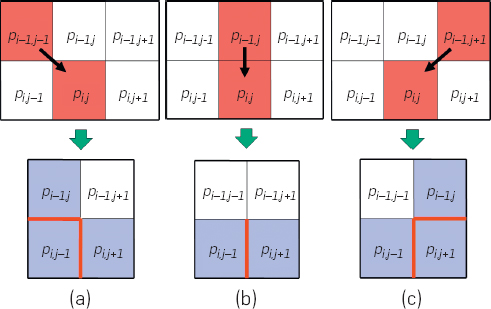
\includegraphics[width=9cm]{cost}
\caption{Possibili scelte per un pixel appartenente al seam}
\label{choice}
\end{figure}

Le funzioni costo relative ai casi $(a),(b)$ e $(c)$ sono definite rispettivamente come: 
\begin{enumerate}[$a$)]
\item $C_{left} (i, j) = |I(i, j + 1) - I(i, j - 1)| + |I(i - 1, j) - I(i, j - 1)| $
\item $C_{up} (i, j) = |I(i, j + 1) - I(i, j - 1)|$
\item $ C_{right} (i, j) = |I(i, j + 1) - I(i, j - 1)| + |I(i - 1, j) - I(i, j + 1)|$
\end{enumerate}

Come nel caso precedente si otterranno valori elevati in presenza di edge; allo stesso tempo, utilizzando la forward energy sarà meno probabile introdurre forti discontinuità che non erano presenti nell'immagine originale, il che rappresenta un notevole vantaggio.

Per identificare un seam ottimale si ricorre alla programmazione dinamica, calcolando una matrice di costo comulativo $M$ (delle stesse dimensioni dell'immagine) in cui ogni entry è ottenuta come segue:
\[
M(i,j) = P(i,j) + min\begin{cases}
 M (i - 1, j - 1) + C_{left} (i, j) \\
 M (i - 1, j) + C_{up}(i, j) \\
 M (i - 1, j + 1) + C_{right}(i, j)\\
\end{cases}
\]
dove $P(i,j)$ può essere usato per aumentare o diminuire il costo di specifici zone dell'immagine secondo diversi criteri; alcuni esempi verranno discussi nella sezione dedicata a object removal e object preservation.

La costruzione di $M$ è di gran lunga l'aspetto più oneroso dell'algoritmo dal punto di vista computazionale in quanto per un'immagine di dimensioni $W \times H$ si ha una complessità di ordine $O(W\times H)$.

Al termine di questa fase si ispeziona l'ultima riga di $M$ e si determina l'indice colonna in corrispondenza del quale si è ottenuto il costo comulativo minimo. Quindi, si ripercorrono a ritroso le righe (prendendo in considerazione solo le 3 entry della riga superiore che sono adiacenti) passando di volta di costo minimo in costo minimo; così facendo, si costruisce un seam la cui energia complessiva è certamente minima. Infine si rimuove il seam appena trovato, ottenendo un' immagine il cui numero di colonne è ridotto di 1. Tale processo è ripetuto finché non si raggiunge la dimensione specificata dall'utente.

\begin{figure}[h]
\centering
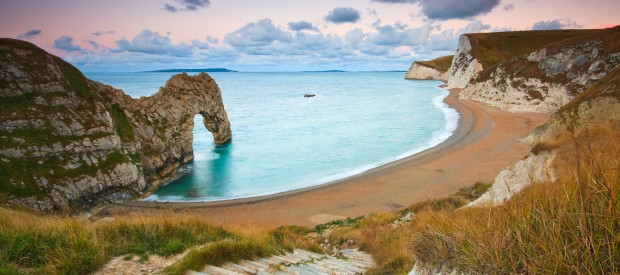
\includegraphics[height=4cm]{coast}
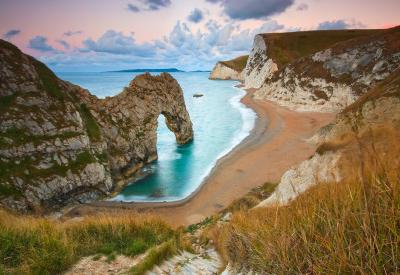
\includegraphics[height=4cm]{coastsmall}
\vskip 0.1cm
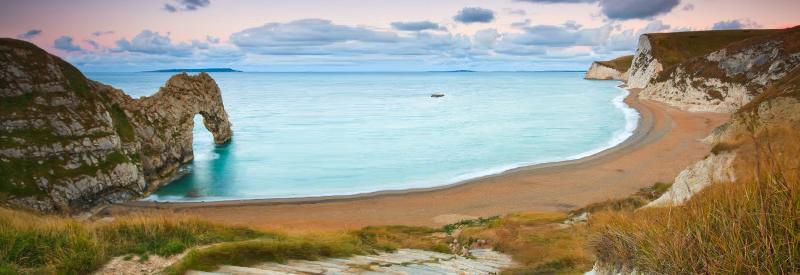
\includegraphics[height=4cm]{coastlarge}
\caption{Immagine originale e rispettivamente ridotta/incrementata di approssimativamente 200 pixel in larghezza.}
\label{preserve}
\end{figure} 
 
 Utilizzando un approccio simile a quello appena discusso è inoltre possibile incrementare il numero di colonne (righe) di un'immagine, piuttosto che ridurlo. Ancora una volta occorre determinare il seam ottimale, ma in questo caso per ciascuna riga si aggiunge un pixel che è la media tra il pixel appartentente al seam e quello alla sua immediata destra (o sinistra). L'inserimento consecutivo di più seam necessita di un'attenzione particolare: infatti, se ad ogni iterazione si prendessero in considerazione tutti i possibili seam dell'immagine appena ottenuta, con grande probabilità il seam avente energia minima sarebbe proprio quello inserito durante l'iterazione precedente, e l'immagine finale risulterebbe distorta come nel caso della figura \ref{bad_insert}. Pertanto se si vuole ottenere un'immagine in cui il numero di colonne sia aumentato di $k$, occorre calcolare una sola volta la matrice $M$ ed in seguito identificare i $k$ seams di costo minore, marcando di volta in volta l'ultimo seam trovato in modo che non possa essere scelto nuovamente. Poiché $M$ viene calcolata un'unica volta, l'operazione di seam insertion risulta notevolmente più veloce rispetto a quella di seam removal.
 \begin{figure}[h]
\centering
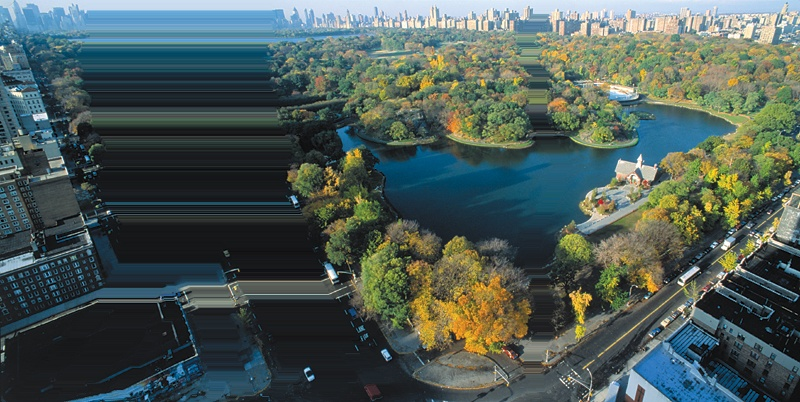
\includegraphics[width=9cm]{insertion}
\caption{Implementazione errata di seam insertion.}
\label{bad_insert}
\end{figure}

\section*{Object removal e object preservation}
Come accennato in precedenza, durante la costruzione della matrice $M$ è possibile utilizzare un parametro $P$ aggiuntivo con lo scopo di assegnare più o meno importanza a determinati pixel, ed avere perciò un maggiore controllo. L'implementazione sfrutta questo parametro permettendo all'utente di rimuovere o al contrario preservare specifici elementi dell'immagine. Attraverso l'uso di semplici maschere si assegnano valori fortemente negativi (nel caso in cui si voglia eliminare un oggetto) oppure molto elevati (nel caso in cui lo si voglia proteggere). Così facendo i seam saranno naturalmente portati ad includere (o ignorare) le zone indicate dalla maschera stessa. Ciò si rivela particolarmente utile se sono presenti elementi la cui eccessiva alterazione risulterebbe evidente e sgradevole, quali volti o figure umane. 

Si può raffinare ulteriormente tale idea sollevando l'utente dal compito di fornire $P$, lasciando tale compito ad una qualche procedura automatica, come un algoritmo di face-detection, o facendo ricorso ad una saliency map. Il secondo dei metodi appena citati, ad esempio, ha portato a buoni risultati in [3] e rappresenta una delle potenziali migliorie da apportare al progetto in futuro. 

I concetti di object removal e object preservation sono illustrati nelle figure che seguono.

\begin{figure}[h]
\centering
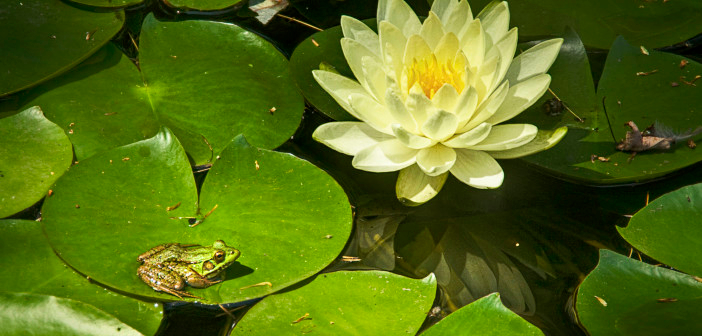
\includegraphics[height=3.5cm]{frog}
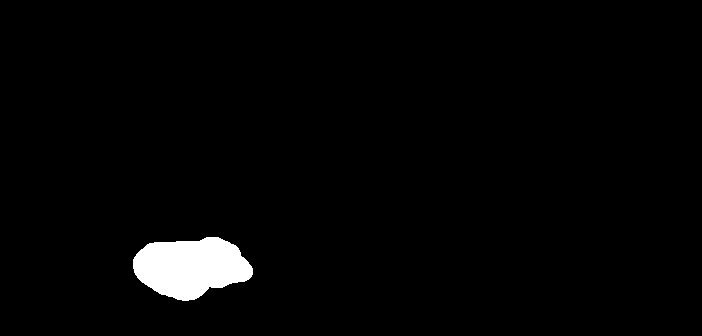
\includegraphics[height=3.5cm]{frogmask}
\vskip 0.1cm
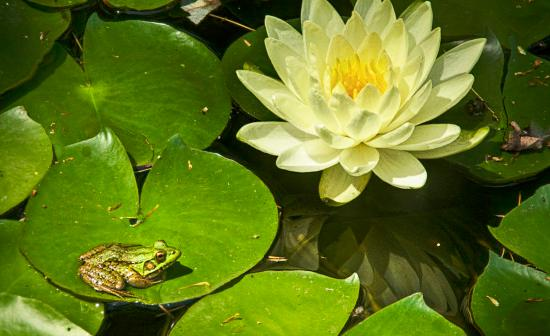
\includegraphics[height=3.5cm]{frogsmall}
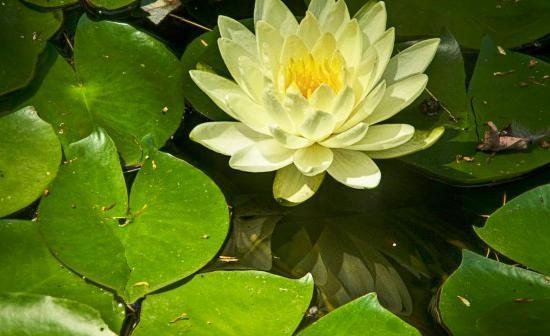
\includegraphics[height=3.5cm]{frogerase}
\caption{L'uso di una maschera di rimozione concentra i seam nella zona dell'oggetto interessato.}
\label{preserve}
\end{figure}
\begin{figure}[h]
\centering
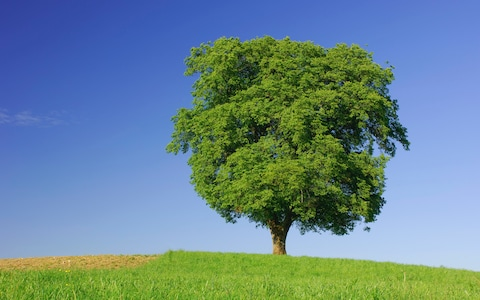
\includegraphics[height=3.5cm]{tree}
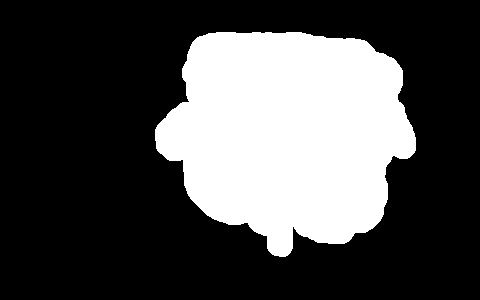
\includegraphics[height=3.5cm]{treemask}
\vskip 0.1cm

\includegraphics[height=3.5cm]{treebad}
\vskip 0.1cm
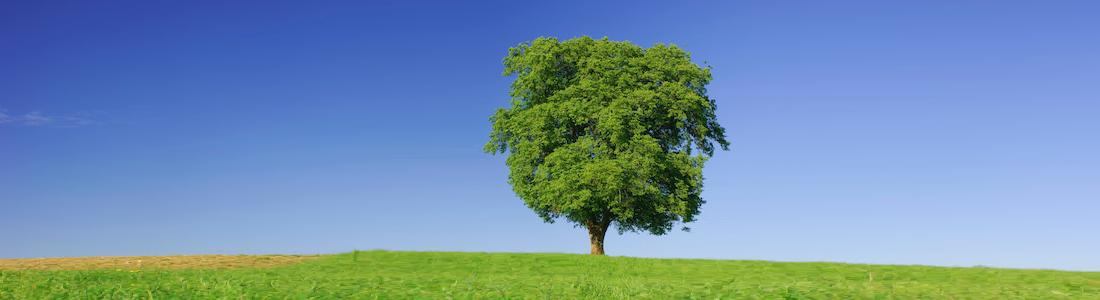
\includegraphics[height=3.5cm]{treegood}
\caption{Immagine la cui larghezza è più che raddoppiata, prima senza e poi con l'uso della maschera di protezione.}
\label{preserve}
\end{figure}

\section*{Osservazioni}
L'operazione di seam carving si rivela poco efficace in presenza di immagini ad alto contenuto informativo, caratterizzate da un grande numero di dettagli in ogni loro parte; in situazioni simili la scelta dei seam ottimali per la rimozione/inserimento è inevitabilmente falsata e spesso porta a risultati insoddisfacenti. Inoltre, se nella scena sono presenti bordi rettilinei che attraversano l'immagine per buona parte della larghezza (altezza) il processo di seam carving tende a generare bordi ``spezzati" con una maggiore probabilità. 
\section*{Bibliografia}
\begin{enumerate}
\item Michael Rubinstein, Ariel Shamir - \textit{Seam carving for content-aware image resizing}
\item Michael Rubinstein, Ariel Shamir, Shai Avidan - \textit{Improved seam carving for video retargeting} 
\item Radhakrishna Achanta, Sabine Süsstrunk - \textit{Saliency detection for content-aware image resizing}
\end{enumerate}
\end{document}
